\begin{center}
    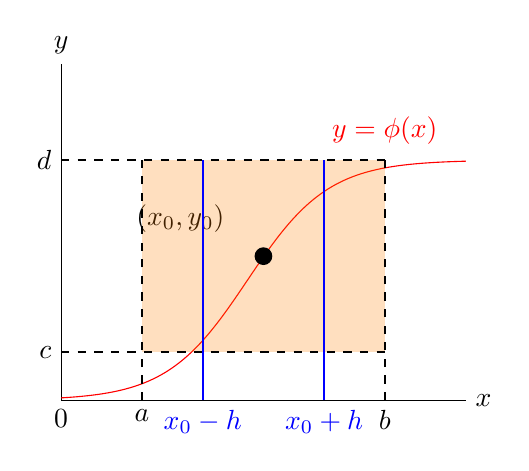
\begin{tikzpicture}
    \begin{axis}[
    scale = 0.75,
    xmin = 0, xmax = 10,
    ymin = 0, ymax = 7,
    axis lines* = left,
    xtick = {0}, ytick = \empty,
    clip = false,
    ]

    % Add plot
    \addplot[domain = 0:10, restrict y to domain = 0:10, samples = 400, color = red]{5/(1+100*e^(-x))};

    % Labels
    \node [right] at (current axis.right of origin) {$x$};
    \node [above] at (current axis.above origin) {$y$};
    \node [below] at (2, 0) {$a$};
    \node [below] at (8, 0) {$b$};

    \node [below, color = blue] at (3.5, 0) {$x_0 - h$};
    \node [below, color = blue] at (6.5, 0) {$x_0 + h$};

    \node [left] at (0, 1) {$c$};
    \node [left] at (0, 5) {$d$};
    
    % mark the centre of rectangle
    \addplot[color = black, mark = *, only marks, mark size = 3pt] coordinates {(5,3)};
    
    % labelling the centre of rectangle
    \node [left = 30pt, above = 5pt] at (5, 3) {$(x_0, y_0)$};
    \node [above = 2pt, color = red] at (8, 5) {$y = \phi (x)$};

    % Colouring areas
    \fill[orange, opacity = 0.25] (2, 1)-- (2, 5) -- (8, 5) -- (8, 1);

    % Dashed lines (y-axis)
    \addplot[color = black, dashed, thick] coordinates {(0, 1) (8, 1)};
    \addplot[color = black, dashed, thick] coordinates {(0, 5) (8, 5)};

    % Dashed lines (x-axis)
    \addplot[color = black, dashed, thick] coordinates {(2, 0) (2, 5)};
    \addplot[color = black, dashed, thick] coordinates {(8, 0) (8, 5)};

    \addplot[color = blue, solid, thick] coordinates {(3.5, 0) (3.5, 5)};
    \addplot[color = blue, solid, thick] coordinates {(6.5, 0) (6.5, 5)};

    \end{axis}
    \end{tikzpicture}
\end{center}